\documentclass[11pt]{article}
\usepackage[utf8]{inputenc}
\usepackage{amsmath}
\usepackage{amsfonts}
\usepackage{amssymb}
\usepackage{bm}
\usepackage{geometry}
\usepackage{graphicx}
\usepackage{xcolor}
\usepackage{booktabs}
\usepackage{algorithm}
\usepackage{algorithmic}

\geometry{margin=0.8in}

\title{Synaptic Depression Modeling \\ Data generation and model fitting}
\author{Jan Balewski, NERSC}
\date{\today}

\begin{document}

\maketitle

\begin{abstract}
We describe a real-time adaptive Bernoulli state-space model (BSSM) for a network of
interacting neurons with short-term synaptic depression (STD) and a lag-$M$ synaptic
memory kernel. The STD mechanism is represented as a latent dynamical resource variable
that is updated at each discrete time step, coupled to observed binary spike indicators
through a Bernoulli likelihood. For context, we also briefly review the Tsodyks--Markram
(TM) resource model, which provides the continuous-time biological foundation for the
discrete STD dynamics used in the BSSM.
\end{abstract}

%=========
\section{Short-Term Synaptic Depression (STD) in Cortical Synapses}
\label{sec:std_intro}

Short-term synaptic depression (STD) is a fast, reversible decrease in synaptic strength
that occurs when a presynaptic cortical neuron fires repeatedly over short time windows
(typically from milliseconds to seconds).

\paragraph{Activity-decaying phenomenon.}
When presynaptic firing is high, the postsynaptic response (EPSCs or IPSCs) becomes
progressively smaller for successive spikes, producing a decaying envelope of synaptic
efficacy during bursts. After presynaptic activity pauses, synaptic strength gradually
recovers to baseline levels.

\paragraph{Main biological mechanism.}
STD is commonly modeled as depletion of synaptic ``resources'' required for effective
neurotransmitter release. At each presynaptic spike, release depends on
(i) the availability of readily releasable vesicles (or release-ready sites) and
(ii) an effective probability of release (often related to intracellular calcium dynamics).
Sustained activity depletes resources and reduces future release, while periods of silence
allow recovery.

\paragraph{Relevant timescales.}
Recovery is typically on intermediate timescales ($\sim 100$\,ms to a few seconds),
depending on synapse type and experimental protocol.

\paragraph{Functional consequences.}
STD acts as a rate-dependent synaptic filter: it attenuates sustained high-rate input,
emphasizes transient changes in firing, and contributes to network stabilization by
preventing runaway excitation.

%=========
\section{Computational Models with STD}
\label{sec:std_models}

We describe two STD frameworks. The TM model (Section~\ref{sec:tm_std}) is included
for conceptual context only. The BSSM (Section~\ref{sec:bssm_std}) is the target
implementation model.

The following notation is shared across both models:
$U\in(0,1]$ is the utilization parameter (fraction of available resources used per spike),
and $\tau_{\mathrm{rec}}$ is the STD recovery time constant.

%=========
\subsection{Tsodyks--Markram (TM) Resource Model: Conceptual Background}
\label{sec:tm_std}

The \emph{Tsodyks--Markram (TM)} model~\cite{Tsodyks1997} is a widely used continuous-time
resource model for \emph{short-term plasticity (STP)}. In the STD-only version, the synapse
has a single \emph{available-resource} variable $x(t)\in[0,1]$. Between presynaptic spikes,
resources recover exponentially:

\begin{figure}[t]
\centering
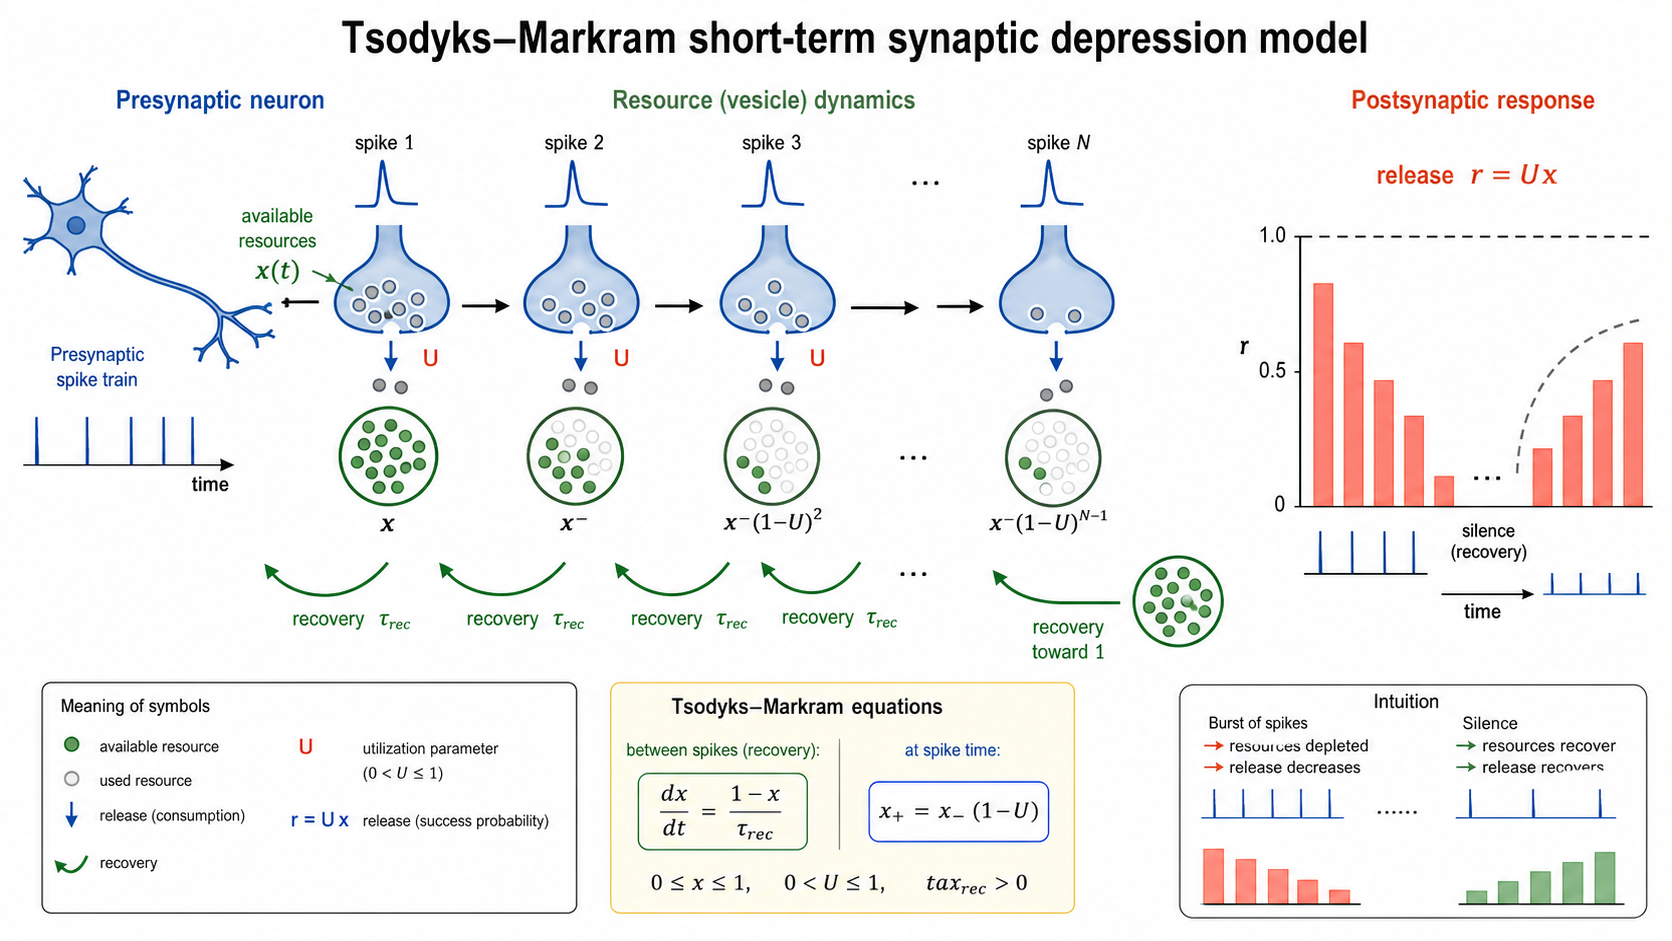
\includegraphics[width=\textwidth]{tm_std_cartoon.png}
\caption{Cartoon of the Tsodyks--Markram STD resource model. Presynaptic spikes
consume a fraction $U$ of the available resource $x$, making successive release
events smaller; during silence, the resource recovers toward $x=1$ with time
constant $\tau_{\mathrm{rec}}$.}
\label{fig:tm_std_cartoon}
\end{figure}

\noindent
The cartoon in Fig.~\ref{fig:tm_std_cartoon} summarizes the STD-only TM mechanism:
spikes multiply the available resource by $(1-U)$, while inter-spike intervals allow
the resource to recover toward one.

\noindent
Between presynaptic spikes,
\begin{equation}
\frac{dx}{dt}=\frac{1-x}{\tau_{\mathrm{rec}}}.
\label{eq:tm_recovery}
\end{equation}
At a presynaptic spike time $t=t_k$, a fraction $U$ of available resources is consumed:
\begin{equation}
x(t_k^+)=x(t_k^-)\,(1-U),
\label{eq:tm_spike_update}
\end{equation}
and the released neurotransmitter amplitude at that spike is
\begin{equation}
r(t_k)=U\,x(t_k^-).
\label{eq:tm_release}
\end{equation}
The TM model provides the biological motivation for the discrete STD resource update
used in the BSSM below (Eq.~\ref{eq:std_ssm_state}), which is the exact discretization
of Eq.~\eqref{eq:tm_recovery} combined with Eq.~\eqref{eq:tm_spike_update}.

\paragraph{Interpretation of $U$.}
The utilization parameter $U$ is a fraction of the resources available at the
moment of a spike, not a fixed fraction of the original full pool. For example,
if $U=0.5$ and several spikes arrive with negligible recovery between them, a
fully recovered synapse releases $0.5$ of the full pool on the first spike,
then $0.25$ on the second, then $0.125$ on the third, and so on. Thus the axon
can still generate more than two closely spaced spikes; STD only makes the
effective synaptic release decrease geometrically during the burst.

\subsection{Real-Time Adaptive Bernoulli State-Space Network Model (BSSM) with STD
            and Lag-$M$ Kernel}
\label{sec:bssm_std}

The \emph{Bernoulli state-space model (BSSM)} represents a network of $N$ neurons using
(i) latent dynamical states encoding STD resources and (ii) a Bernoulli observation model
for binary spike indicators conditioned on those states. This is the primary model of
interest. At physiological firing rates ($30$--$50$\,Hz) and bin width
($\Delta t = 1$\,ms), the per-bin spike probability is
$p \approx r\Delta t = 0.03$--$0.05$. The corresponding Poisson probability
of two or more spikes in one bin is approximately $p^2/2$, ranging from
$4.5\times10^{-4}$ to $1.25\times10^{-3}$. Thus the Bernoulli model is a good
approximation for binary spike indicators while explicitly enforcing at most one
spike per bin.

\begin{figure}[t]
\centering
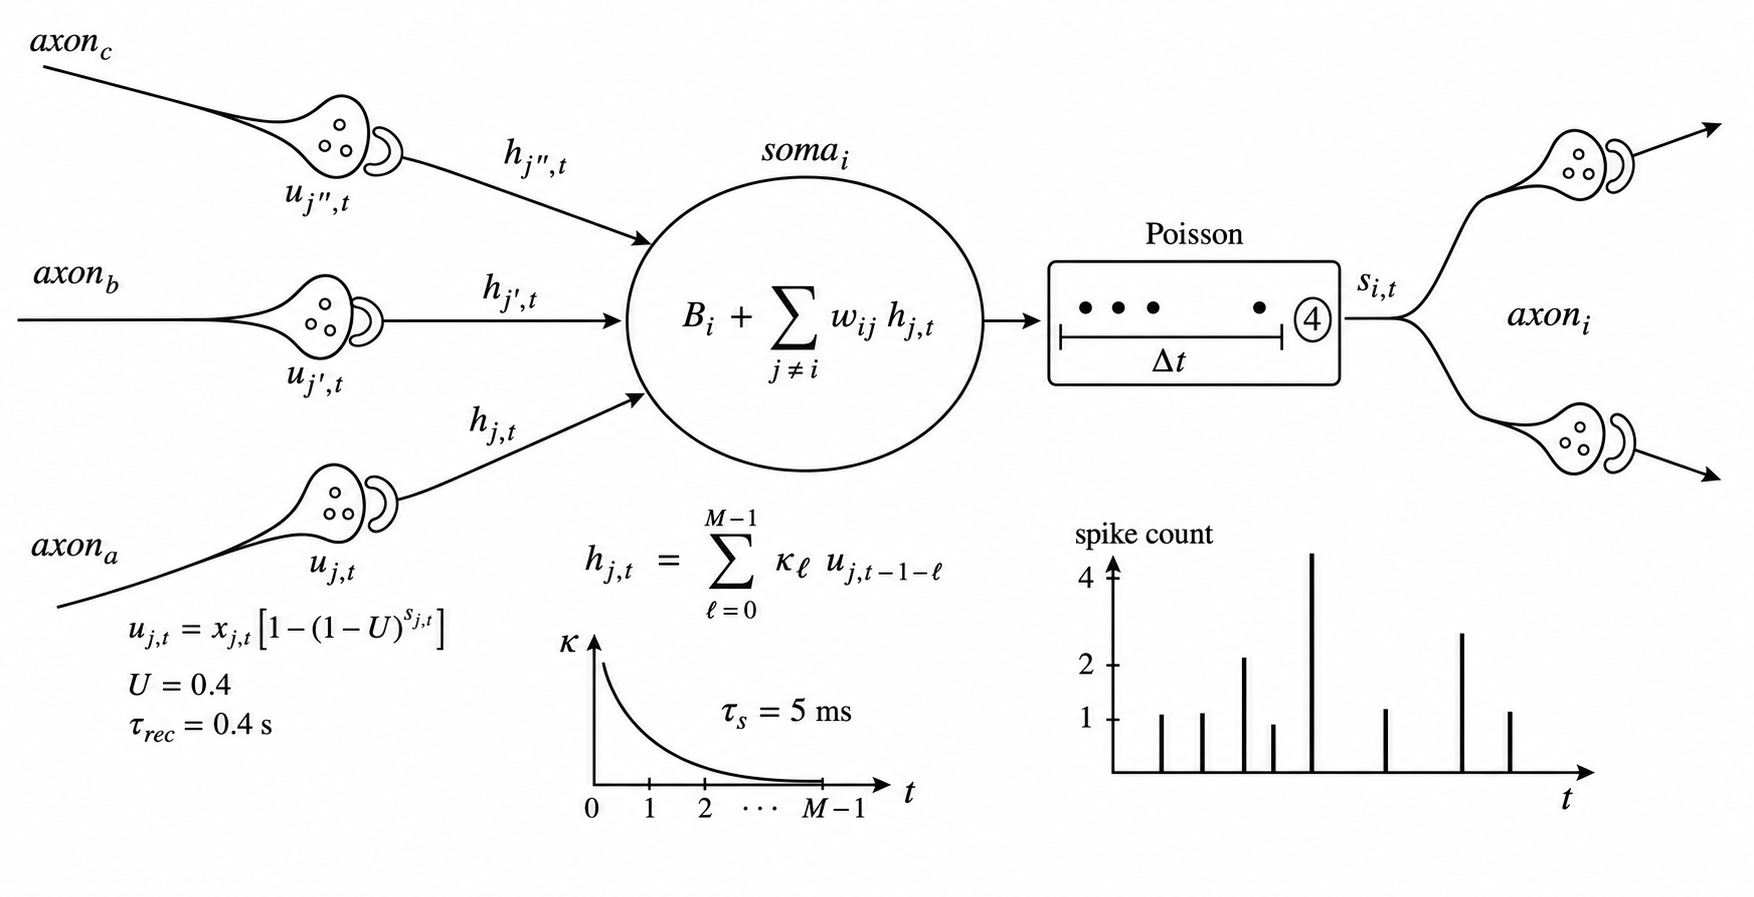
\includegraphics[width=\textwidth]{bssm_std_model_cartoon.png}
\caption{Cartoon of the full BSSM with STD and a lag-$M$ synaptic kernel.
Presynaptic binary spikes $s_{j,t}$ modulate the latent resource $x_{j,t}$,
produce STD-weighted release $u_{j,t}$, pass through a causal synaptic kernel to
form filtered drive $h_{j,t}$, and enter the postsynaptic Bernoulli observation
model through signed recurrent weights $W_{ij}$ and baseline $b_i$.}
\label{fig:bssm_std_cartoon}
\end{figure}

\noindent
Figure~\ref{fig:bssm_std_cartoon} summarizes the sequential data-flow view of
the model: the recurrent weighted input determines the postsynaptic spike
probability, sampled presynaptic spikes generate release from the current STD
resource, and that release updates both the next STD state and the filtered
drive available in the next bin.

\paragraph{Discrete time and notation.}
Let $t\in\{0,1,\dots,T-1\}$ index time bins of width $\Delta t$.
For each neuron $j$, the primary observable is the binary \emph{spike indicator}
\begin{equation}
s_{j,t} =
\begin{cases}
1 & \text{neuron } j \text{ fired a spike in bin } t,\\
0 & \text{neuron } j \text{ was silent in bin } t,
\end{cases}
\end{equation}
which records only \emph{whether} a spike occurred. The downstream efficacy of that
spike is determined separately by the latent STD resource variable $x_{j,t}\in[0,1]$,
which encodes the fraction of neurotransmitter available for release at the start of
bin $t$ (see Eq.~\ref{eq:std_ssm_state}). A spike that occurs when resources are
depleted ($x_{j,t}\approx 0$) contributes little to postsynaptic drive, whereas a
spike after full recovery ($x_{j,t}\approx 1$) contributes maximally.

\paragraph{STD latent state dynamics.}
Each presynaptic neuron $j$ has its own latent resource variable $x_{j,t}$,
tracking the STD state of that neuron's outgoing synapses independently of all
other neurons. The full network state is the collection $\{x_{j,t}\}_{j=1}^{N}$,
with each variable evolving as the exact discretization of the TM continuous-time
recovery (Eq.~\ref{eq:tm_recovery}) combined with spike-triggered consumption
(Eq.~\ref{eq:tm_spike_update}):
\begin{equation}
\begin{aligned}
x^{\mathrm{dep}}_{j,t}
&=
\underbrace{x_{j,t}\big(1-U\,s_{j,t}\big)}_{\text{spike-triggered depletion}},
\\
x_{j,t+1}
&=
\underbrace{1-\big(1-x^{\mathrm{dep}}_{j,t}\big)
e^{-\Delta t/\tau_{\mathrm{rec}}}}_{\text{exponential recovery after depletion}},
\qquad j=1,\dots,N .
\end{aligned}
\label{eq:std_ssm_state}
\end{equation}
Release during bin $t$ uses the pre-spike resource $x_{j,t}$. If a spike occurs,
a fraction $U$ is first consumed, and the depleted resource then recovers toward
$1$ over the interval to bin $t+1$. Because the update depends only on neuron
$j$'s own spike indicator, resource variables of different neurons are
conditionally independent given their respective spike histories, allowing all
$N$ updates to proceed in parallel.

\paragraph{STD-modulated release.}
The effective synaptic release from neuron $j$ in bin $t$ is:
\begin{equation}
u_{j,t}=U\,x_{j,t}\,s_{j,t}.
\label{eq:std_release}
\end{equation}
This quantity is zero in the absence of a spike, small when resources are depleted
by recent activity, and large (up to $U$) after full recovery.

\paragraph{Lag-$M$ synaptic kernel.}
Synaptic currents have temporal extent beyond a single bin. We convolve the
STD-modulated release with a causal lag-$M$ kernel
$\bm{\kappa}=(\kappa_1,\dots,\kappa_M)^\top$, $\kappa_\ell\geq 0$, encoding how
a release event at lag $\ell$ bins contributes to postsynaptic drive at time $t$.
The effective STD-filtered synaptic input from neuron $j$ at time $t$ is:
\begin{equation}
h_{j,t} = \sum_{\ell=1}^{M}\kappa_\ell\,u_{j,t-\ell}.
\label{eq:lag_kernel}
\end{equation}
Here $M\Delta t$ is the finite lag-history span for the fast synaptic current.
For an exponential synaptic kernel, practical choices take $M\Delta t$ to be
several synaptic time constants $\tau_s$ so that the current tail is small at
the truncation boundary. This lag window is distinct from the STD recovery
memory: the slower recovery governed by $\tau_{\mathrm{rec}}$ is carried by the
latent state $x_{j,t}$ rather than by the finite synaptic kernel. Practical
kernel choices include exponential decay, raised cosine basis functions, or a
free learnable filter (see Section~\ref{sec:gen_kernel} for the generator
choice).

\paragraph{Bernoulli observation model.}
For each postsynaptic neuron $i$, the conditional spiking probability is:
\begin{equation}
p_{i,t}
=
\sigma\!\left(
b_i
+
\sum_{\substack{j=1\\j\neq i}}^{N}
W_{ij}\,h_{j,t}
\right),
\label{eq:bernoulli_obs}
\end{equation}
where $\sigma(z)=1/(1+e^{-z})$ is the logistic sigmoid, $b_i$ is a baseline
log-odds for neuron $i$, and $W_{ij}$ is the synaptic weight from neuron $j$
to neuron $i$ (positive for excitatory, negative for inhibitory connections).
Self-connections are excluded by the constraint $j\neq i$.
The spike indicator is then drawn as:
\begin{equation}
s_{i,t} \sim \mathrm{Bernoulli}(p_{i,t}).
\label{eq:bernoulli_likelihood}
\end{equation}
For $t-\ell<0$, pre-history values $u_{j,t-\ell}$ are set to zero, corresponding
to a fully recovered synapse with no prior spiking.

\paragraph{Summary of model parameters.}
The full parameter set of the BSSM is $\theta=\{b_i, W_{ij}, \kappa_\ell, U,
\tau_{\mathrm{rec}}\}$, where $b_i$ and $W_{ij}$ are neuron- and synapse-specific,
while this model assumes a single shared utilization parameter $U$ for all
presynaptic neurons and outgoing synapses. The recovery time
$\tau_{\mathrm{rec}}$ is also treated as shared in the generator and estimation
procedure below. In the generator
(Section~\ref{sec:generator}), all parameters are fixed to known ground-truth
values; in inference, they constitute the quantities to be estimated.

\paragraph{Real-time and adaptive aspects.}
The term \emph{real-time} refers to the fact that both the latent STD state
$x_{j,t}$ and parameter estimates can be updated sequentially as new spike
indicators $s_{i,t}$ arrive, without reprocessing the full data history. The term
\emph{adaptive} refers to the property that $x_{j,t}$ automatically tracks recent
presynaptic spiking through Eq.~\eqref{eq:std_ssm_state}: resources deplete during
bursts and recover during silence, so the effective synaptic gain $u_{j,t}$ adapts
online to the presynaptic firing history. Together, these properties make the BSSM
suitable for closed-loop neural decoding or real-time inference scenarios.

%=========
\section{Data Generator:  Cortical Network with STD}
\label{sec:generator}

To validate the BSSM and test inference procedures, we generate synthetic spike
trains from a network that mimics key properties of mammalian cortical dynamics.
The generator uses the same BSSM structure as the inference model 
(Section~\ref{sec:bssm_std}), but with all parameters fixed to known ground-truth
values, enabling direct comparison between true and estimated quantities.

%=========
\subsection{Network Architecture}
\label{sec:gen_architecture}

We consider a network of $N\in[50, 500]$ neurons partitioned following Dale's law
into $N_E = 0.8\,N$ excitatory and $N_I = 0.2\,N$ inhibitory neurons.
The code constructs the initial synaptic matrix $W\in\mathbb{R}^{N\times N}$
with a spatial connections Dale generator. Neurons are
placed on a two-dimensional grid over $[0,L]\times[0,H]$ with minimum spacing
$d_{\min}$, and their order is sorted by position. For each presynaptic neuron
$j$, an out-degree $k_j$ is drawn from the configured range and $k_j$ distinct
postsynaptic targets are sampled without replacement with probability
proportional to $D_{ij}^{-\delta}$, excluding $i=j$. This gives nearby neurons
higher connection probability while keeping the diagonal zero.

The nonzero weights obey Dale's law column-by-column:
\begin{equation}
W^{(0)}_{ij} =
\begin{cases}
+a_{ij} & \text{if neuron } j \text{ is excitatory},\\
-\frac{N_E}{N_I}\,a_{ij} & \text{if neuron } j \text{ is inhibitory},
\end{cases}
\qquad
a_{ij}\sim\mathrm{Uniform}(1-v,1+v),
\label{eq:weight_draw}
\end{equation}
for sampled edges only, with $W^{(0)}_{ii}=0$. Finally, the whole matrix is
rescaled to the requested spectral radius $R$,
\begin{equation}
W = W^{(0)}\,\frac{R}{\rho(W^{(0)})},
\label{eq:weight_matrix}
\end{equation}
which preserves sparsity, signs, Dale's law, and the zero diagonal.


%=========
\subsection{Synaptic Kernel}
\label{sec:gen_kernel}

We use an \emph{exponential decay kernel} as the ground-truth synaptic filter:
\begin{equation}
\kappa_\ell = (1-\alpha)\,\alpha^{\ell-1}, \qquad \ell = 1,\dots,M,
\label{eq:exp_kernel}
\end{equation}
where $\alpha = e^{-\Delta t/\tau_s}$ and $\tau_s$ is the synaptic time constant.
This kernel corresponds to a standard single-compartment synaptic current model
and is the exact discrete-time analog of the continuous-time shot-noise synaptic
model. It is normalized so that $\sum_{\ell=1}^{M}\kappa_\ell \approx 1$ for
$M\Delta t \gg \tau_s$.

A key computational advantage of this choice is that the lag-$M$ convolution
in Eq.~\eqref{eq:lag_kernel} can be evaluated by a tail-corrected recursive
update:
\begin{equation}
h_{j,t+1}
=
\alpha\,h_{j,t} + (1-\alpha)\,u_{j,t}
-
(1-\alpha)\alpha^{M}\,u_{j,t-M},
\label{eq:recursive_kernel}
\end{equation}
with $u_{j,t-M}=0$ when $t-M<0$. This recurrence is exactly equivalent to the
finite lag-$M$ convolution for the exponential kernel and avoids explicitly
summing over all $M$ lags at every time step. The decay rate of $\kappa_\ell$
is set by the fast synaptic time constant $\tau_s$, whereas the slower STD time
constant $\tau_{\mathrm{rec}}$ enters through the latent state update in
Eq.~\eqref{eq:std_ssm_state}.

%=========
\subsection{Ground-Truth Parameter Values}
\label{sec:gen_params}

Table~\ref{tab:gen_params} lists the ground-truth parameter values used in the
generator, motivated by mammalian cortical physiology.

\begin{table}[h]
\centering
\small
\setlength{\tabcolsep}{3pt}
\begin{tabular}{@{}llll@{}}
\toprule
Parameter & Symbol & Value & Rationale \\
\midrule
Time bin width         & $\Delta t$            & $1$\,ms                           & Resolves spikes; keeps $p$ small \\
Synaptic time constant & $\tau_s$              & $3$--$5$\,ms                      & AMPA-like fast excitation \\
STD recovery time      & $\tau_{\mathrm{rec}}$ & $200$--$500$\,ms                  & Typical cortical STD \\
Utilization parameter  & $U$                   & $0.3$--$0.5$                      & Shared moderate depression \\
Weight scale           & $v, R$                & $v=0.4,\ R=0.90$                  & Spectral-radius scaling \\
Baseline log-odds      & $b_i$                 & sampled idle-rate range           & User-adjusted baseline drive \\
Kernel length          & $M$                   & $\gtrsim 3$--$5\,\tau_s/\Delta t$ & Fast synaptic lag window \\
\bottomrule
\end{tabular}
\caption{Ground-truth generator parameters. Ranges reflect variability across
synapse types and network sizes. The kernel length $M$ controls the finite lag
history for the fast synaptic filter and is separate from the STD recovery time
$\tau_{\mathrm{rec}}$. The baseline $b_i$ is expressed as a log-odds consistent
with the Bernoulli observation model (Eq.~\ref{eq:bernoulli_obs}).}
\label{tab:gen_params}
\end{table}

%=========
\subsection{Generation Procedure}
\label{sec:gen_procedure}

Given the fixed parameters, synthetic spike indicators are generated sequentially
for $t = 0, 1, \dots, T-1$ as follows.

\begin{algorithm}
\caption{Synthetic network spike train generator}
\label{alg:generator}
\begin{algorithmic}[1]
\STATE \textbf{Initialize:} $x_{j,0} \leftarrow 1$ for all $j$ (fully recovered);
       $h_{j,0} \leftarrow 0$ and $u_{j,t}\leftarrow0$ for $t<0$; draw $W$, $\{b_i\}$ as in
       Eqs.~\eqref{eq:weight_draw}--\eqref{eq:weight_matrix}.
\FOR{$t = 0, 1, \dots, T-1$}
  \FOR{each neuron $i = 1,\dots,N$}
    \STATE Compute spiking probability:
           $p_{i,t} \leftarrow \sigma\!\left(b_i +
           \sum_{j \neq i} W_{ij}\,h_{j,t}\right)$
           \hfill(Eq.~\ref{eq:bernoulli_obs})
    \STATE Draw spike indicator:
           $s_{i,t} \sim \mathrm{Bernoulli}(p_{i,t})$
           \hfill(Eq.~\ref{eq:bernoulli_likelihood})
  \ENDFOR
  \FOR{each neuron $j = 1,\dots,N$}
    \STATE Compute STD-modulated release from pre-spike resources:
           $u_{j,t} \leftarrow U\,x_{j,t}\,s_{j,t}$
           \hfill(Eq.~\ref{eq:std_release})
    \STATE Update STD resource:
           $x_{j,t+1} \leftarrow
           1-\big(1-x_{j,t}(1-U\,s_{j,t})\big)e^{-\Delta t/\tau_{\mathrm{rec}}}$
           \hfill(Eq.~\ref{eq:std_ssm_state})
    \STATE Update recursive synaptic filter:
           $h_{j,t+1} \leftarrow
           \alpha h_{j,t} + (1-\alpha)u_{j,t}
           -(1-\alpha)\alpha^M u_{j,t-M}$
           \hfill(Eq.~\ref{eq:recursive_kernel})
  \ENDFOR
\ENDFOR
\STATE \textbf{Output:} spike indicators $\{s_{j,t}\}$, ground-truth STD states
       $\{x_{j,t}\}$, weight matrix $W$.
\end{algorithmic}
\end{algorithm}

%=========
\subsection{Network Stability Check}
\label{sec:gen_stability}

With recurrent excitatory connections, the network can exhibit runaway activity
if synaptic weights are too large. Before generating long recordings, we recommend
a short pilot run ($\sim 1$\,s) and verification that mean firing rates across
neurons remain in the target range of $30$--$50$\,Hz. If rates exceed this
range, one should reduce the spectral-radius target $R$ or increase $U$: stronger
STD provides a natural activity-dependent stabilizing mechanism by reducing
synaptic efficacy during high-rate episodes.

%=========
\section{Initializing $U$ from Raw Spike Data}
\label{sec:U_estimation}

The utilization parameter $U$ controls the multiplicative depletion of synaptic
resources at each presynaptic spike. Because this depletion affects the relative
release generated by consecutive spikes from the same neuron, tight-pair
statistics provide a useful initializer for the network-wide $U$. In this
section, $U$ denotes the true or model utilization, while $\tilde{U}$ denotes an
inferred value obtained from data. This raw
estimate is not treated as final: it is refined later by likelihood optimization
together with $\tau_\text{rec}$ and the recurrent parameters. We do not attempt
to pre-estimate $\tau_\text{rec}$ from raw consecutive-spike ISIs: at the target
30--50~Hz rates, typical ISIs are tens of milliseconds, much shorter than the
expected 0.2--0.5~s recovery time. Instead, $\tau_\text{rec}$ is treated as
unknown and initialized from a fixed physiological guess in the full fitting
procedure. This section estimates the recording requirements for the raw
$\tilde{U}$ initializer.

\subsection{The Burst-Pair Estimator for $U$}

Consider two consecutive spikes from presynaptic neuron $j$, separated by an
inter-spike interval (ISI) $\delta$. Let $x_1^-$ be the resource immediately
before the first spike. After spike-triggered depletion and recovery toward
one, the resource immediately before the second spike is
%
\begin{equation}
    x_2^- = 1 - \left(1 - x_1^-(1-U)\right)e^{-\delta/\tau_\text{rec}}.
    \label{eq:pair_recovery}
\end{equation}
%
For this pair, define the two release amplitudes by the same rule as
Eq.~\eqref{eq:std_release}: $u_1=U x_1^-$ for the first spike and
$u_2=U x_2^-$ for the second spike. The ratio of second-spike to first-spike
release is therefore
%
\begin{equation}
    \rho(\delta) = \frac{u_2}{u_1}
    =
    (1-U)e^{-\delta/\tau_\text{rec}}
    + \frac{1-e^{-\delta/\tau_\text{rec}}}{x_1^-}.
    \label{eq:rho_estimator}
\end{equation}
%
In the linear-response regime, $\rho(\delta)$ can be estimated from the ratio of
postsynaptic excess firing probabilities above baseline in the bins following
the first and second presynaptic spikes. The key point is that the zero-ISI
limit is independent of the unknown starting resource:
%
\begin{equation}
    \lim_{\delta\to0^+}\rho(\delta)=1-U.
    \label{eq:rho_zero_isi}
\end{equation}
%
Thus the estimator does not require a long silent period before the tight pair.
It requires the pair itself to be sufficiently tight that recovery during the
ISI is negligible. For finite $\delta$, the recovery correction depends on the
unknown $x_1^-$; depleted states amplify the bias. A practical approximation is
to replace $x_1^-$ by the stationary mean resource expected at the observed
presynaptic firing rate $r$:
%
\begin{equation}
    \bar{x}(r,U,\tau_\text{rec})
    \approx
    \frac{1}{1+U r \tau_\text{rec}},
    \label{eq:xbar_stationary}
\end{equation}
%
which follows by balancing recovery toward one against average spike-triggered
depletion. Substituting $\bar{x}$ into Eq.~\eqref{eq:rho_estimator} gives an
average finite-ISI correction. To make the bias explicit, define the naive
zero-ISI inferred value $\tilde{U}_0(\delta)=1-\hat{\rho}(\delta)$. The
finite-ISI effect is an additive bias in the inferred utilization, not a
multiplicative rescaling. Its
magnitude is approximately
%
\begin{equation}
    B_U(\delta)
    \equiv
    \left|\tilde{U}_0(\delta)-U\right|
    \approx
    \left(1-e^{-\delta/\tau_\text{rec}}\right)
    \left[
        \frac{1}{\bar{x}(r,U,\tau_\text{rec})}-(1-U)
    \right]
    \sim
    \frac{1-e^{-\delta/\tau_\text{rec}}}{\bar{x}(r,U,\tau_\text{rec})},
    \label{eq:U_bias}
\end{equation}
%
so high firing rates, which reduce $\bar{x}$, require tighter ISI windows. Let
$\varepsilon_U$ denote the allowed additive bias in the inferred utilization
$\tilde{U}$. In continuous time, keeping this finite-ISI correction below
$\varepsilon_U$ would require an ideal small-window cutoff
%
\begin{equation}
    \delta_\text{ideal}
    \approx
    \frac{\varepsilon_U\,\tau_\text{rec}}
    {\frac{1}{\bar{x}(r,U,\tau_\text{rec})}-(1-U)},
    \label{eq:delta_ideal}
\end{equation}
%
valid when $\delta_\text{ideal}\ll\tau_\text{rec}$. With 1~ms binned spike
trains, however, the smallest resolvable nonzero ISI is one time bin. Therefore
the practical tight-pair cutoff used for initialization is
%
\begin{equation}
    \delta_\text{max}=\Delta t=1~\mathrm{ms}.
    \label{eq:delta_max}
\end{equation}
%
This cutoff is not chosen because it makes the finite-ISI bias vanish; it is the
finest window available in the sampled data. The typical ISI,
$1/r\approx20$--$33$~ms, is much too large to use as a tight-pair cutoff because
recovery during that interval is no longer negligible. Because
$\bar{x}$ itself depends on the unknown $U$, this raw estimator is naturally
iterative in $\tilde{U}$: start from a nominal value (for example
$\tilde{U}=0.5$), compute $\bar{x}(r,\tilde{U},\tau_\text{rec})$ and
$\delta_\text{max}$, estimate a new $\tilde{U}$ from the selected tight pairs,
then update $\bar{x}$ and repeat until the initializer stabilizes.

With a nominal or current estimate of $\tau_\text{rec}$ and an average resource
estimate $\bar{x}$, each observed ratio can be corrected before averaging:
%
\begin{equation}
    \tilde{U}_\text{corrected}(\delta,\bar{x})
    =
    1 -
    e^{\delta/\tau_\text{rec}}
    \left[
        \hat{\rho}(\delta) - \frac{1-e^{-\delta/\tau_\text{rec}}}{\bar{x}}
    \right].
    \label{eq:U_correction}
\end{equation}
%
The tight-pair window is still useful after this correction because it limits
sensitivity to model mismatch, refractory effects, and finite-sample noise in
the excess-probability ratio. In the protocol below, the raw tight-pair estimate
is used only to initialize $\tilde{U}$; the final value is obtained by likelihood
optimization.

\paragraph{Treatment of $\tau_\text{rec}$ during initialization.}
The tight-pair initializer requires a value of $\tau_\text{rec}$ in
Eqs.~\eqref{eq:xbar_stationary}--\eqref{eq:U_correction}, but raw spike pairs do
not give a practical standalone estimate of this slow time constant at the
target rates. Therefore the initialization uses a fixed physiological guess,
for example $\tilde{\tau}_\text{rec}^{(0)}=0.4$~s. This value is not assumed to
be correct. It only sets the initial resource scale and tight-pair window; the
three-block likelihood optimization later updates $\tilde{\tau}_\text{rec}$
directly in Block~C.

\subsection{Statistical Requirements: Tight Pairs and Shots}
\label{sec:tight_pairs_shots}

\textbf{Tight pairs} are consecutive spike pairs from the same neuron with
ISI $\delta \leq \delta_\text{max}$. For a Poisson spike train with rate $r$
observed for duration $T_\text{obs}=T\Delta t$, the expected number of tight
pairs per neuron is
%
\begin{equation}
    \mathcal{P}_\text{pairs}
    = r T_\text{obs}\left(1-e^{-r\delta_\text{max}}\right)
    \approx r^2 T_\text{obs}\delta_\text{max},
    \label{eq:Npairs}
\end{equation}
%
with the approximation valid only when $r\delta_\text{max}\ll1$. Thus the
physical recording duration, firing rate, and coincidence window determine the
pair count; the time bin width matters only insofar as it must resolve the
selected ISIs.

\textbf{Shots} are the postsynaptic spike observations that follow selected
tight-pair events. Since the model uses one shared $U$, tight pairs pool across
all presynaptic neurons. If the mean number of true postsynaptic targets per
presynaptic neuron is $k$, the approximate number of informative shots is
%
\begin{equation}
    N_\text{shots}^\text{eff}
    \approx N\,\mathcal{P}_\text{pairs}\,k.
    \label{eq:Nshots}
\end{equation}
%
The raw data contain observations from all possible postsynaptic neurons, but
only the connected targets contribute coherent signal to the excess-probability
ratio. A rough precision target is
$N_\text{shots}^\text{eff}\gtrsim 1/\varepsilon_U^2$. For
$N=500$ and $k=75$, even $\mathcal{P}_\text{pairs}=10$ per neuron gives
$3.75\times10^5$ effective shots, so the estimator is usually limited more by
the recovery-bias window than by shot noise.

\subsection{Parameter Dependence and Operating Points}

With the stationary-resource approximation, the ideal continuous-time
coincidence window is set by the additive-bias tolerance in
Eq.~\eqref{eq:delta_ideal}. In the actual 1~ms binned data, sub-millisecond
windows cannot be resolved, so the practical choice is fixed to
$\delta_\text{max}=1$~ms. Higher firing rates reduce $\bar{x}$ and therefore
increase the implied finite-ISI bias, but they also increase the number of
available tight pairs. The typical ISI, $1/r$, should not be used as a
tight-pair cutoff: for $r=30$~Hz it is about 33~ms, which would introduce an
additive bias of order $0.5$ in $\tilde{U}$ under the baseline parameters.

\begin{table}[h]
\centering
\caption{Practical tight-pair statistics for true/nominal $U=0.5$,
$\delta_\text{max}=\Delta t$, $N=500$, mean out-degree $k=0.15N=75$, and fixed
recording duration $T_\text{obs}=1000$~s. $B_U(\delta)$ is the implied additive
finite-ISI bias from Eq.~\ref{eq:U_bias}, evaluated at $\delta=\Delta t$; for
the 1~ms rows this is $B_U(1~\mathrm{ms})$. $\mathcal{P}_\text{pairs}$ uses the
exact Poisson expression in Eq.~\ref{eq:Npairs}. The resource mean $\bar{x}$ is
computed from Eq.~\ref{eq:xbar_stationary}. Baseline row in bold.}
\label{tab:tight_pairs}
\setlength{\tabcolsep}{4pt}
\begin{tabular}{clcccccc}
\toprule
Row & Description & $\Delta t$ & $r$ & $\tau_\text{rec}$ &
$\bar{x}$ & $B_U(\Delta t)$ & $\mathcal{P}_\text{pairs}$/neuron \\
 & & (ms) & (Hz) & (s) & & & \\
\midrule
\textbf{1} & \textbf{Baseline} & \textbf{1} & \textbf{30} & \textbf{0.4} & \textbf{0.143} & \textbf{0.016} & \textbf{887} \\
2 & Baseline, finer bin & 0.5 & 30 & 0.4 & 0.143 & 0.008 & 447 \\
3 & Higher target rate & 1 & 50 & 0.4 & 0.091 & 0.026 & 2,439 \\
4 & Higher target rate, finer bin & 0.5 & 50 & 0.4 & 0.091 & 0.013 & 1,235 \\
5 & Short $\tau_\text{rec}$ & 1 & 30 & 0.2 & 0.250 & 0.017 & 887 \\
6 & Short $\tau_\text{rec}$, finer bin & 0.5 & 30 & 0.2 & 0.250 & 0.009 & 447 \\
7 & Long $\tau_\text{rec}$ & 1 & 30 & 0.5 & 0.118 & 0.016 & 887 \\
8 & Long $\tau_\text{rec}$, finer bin & 0.5 & 30 & 0.5 & 0.118 & 0.008 & 447 \\
\bottomrule
\end{tabular}
\end{table}

The main conclusion from Table~\ref{tab:tight_pairs} is that, for the
$N=500$ network considered here, network-wide pooling gives ample effective
shots throughout the 30--50~Hz target firing range even when only one-bin
tight pairs are used. The cost is a percent-level finite-ISI bias in the raw
$\tilde{U}$ initializer. This is acceptable for initialization because the
three-block likelihood fit subsequently refines $\tilde{U}$; it would not be
acceptable as a final standalone estimator.




%=========
\section{Summary of the Parameter Estimation Method}
\label{sec:param_estimation}

The true BSSM parameter set is
$\theta = \{b_i, W_{ij}, \tau_\text{rec}, U, \tau_s\}$. The corresponding
estimated parameter set is denoted
$\tilde{\theta} = \{\tilde{b}_i, \tilde{W}_{ij}, \tilde{\tau}_\text{rec},
\tilde{U}\}$, with $\tau_s$ assumed known from the fast synaptic time scale or
fixed by the chosen kernel. The utilization estimate $\tilde{U}$ is initialized
from tight pairs using a nominal recovery time, while
$\tilde{\tau}_\text{rec}$ is treated as unknown and initialized from a fixed
physiological guess, $\tilde{\tau}_\text{rec}^{(0)}=0.4$~s; neither is fixed
thereafter.
The final estimate is obtained by a three-block coordinate-descent
maximum-likelihood procedure over $\{\tilde{b}_i,\tilde{W}_{ij}\}$,
$\tilde{U}$, and $\tilde{\tau}_\text{rec}$.

\subsection{Pre-processing: Initializing $\tilde{\tau}_\text{rec}$ and Estimating $\tilde{U}$}

\textbf{Step 1 --- Initialize $\tilde{\tau}_\text{rec}$.} Do not pre-estimate
$\tau_\text{rec}$ from raw consecutive-spike ISIs. At 30--50~Hz, typical ISIs
are only $20$--$33$~ms, so they do not span the 0.2--0.5~s recovery range
needed for a stable standalone estimate. Set a physiological starting value,
\begin{equation}
    \tilde{\tau}_\text{rec}^{(0)} = 0.4~\text{s}.
\end{equation}
This value is only an initialization for the forward STD recursion and for the
tight-pair correction; it is updated later in Block~C.

\textbf{Step 2 --- Initialize $\tilde{U}$ iteratively.} Estimate
$\tilde{U}^{(0)}$ from the
tight-pair release ratio in Eq.~\eqref{eq:rho_estimator}, pooling pairs across
all presynaptic neurons. Because the finite-ISI correction depends on the
typical pre-pair resource level, and that resource level depends on $U$, this
initialization is a fixed-point procedure rather than a one-pass calculation.
Start from a nominal value, for example $\tilde{U}=0.5$; compute
$\bar{x}(r,\tilde{U},\tilde{\tau}_\text{rec}^{(0)})$ from
Eq.~\eqref{eq:xbar_stationary}; set the tight-pair window using
Eq.~\eqref{eq:delta_max}; estimate a new $\tilde{U}$ using the corrected ratio
in Eq.~\eqref{eq:U_correction}; then recompute $\bar{x}$ and repeat until the
update changes negligibly. With an extremely narrow coincidence window, the
zero-ISI approximation $\lim_{\delta\to0^+}\rho(\delta)=1-U$ is recovered as
the limiting case. This estimate anchors the subsequent optimization but is
allowed to move during the likelihood fit.

\textbf{Step 3 --- Initialize $\{b_i, W_{ij}\}$.} Given
$\tilde{\tau}_\text{rec}^{(0)}$ and $\tilde{U}^{(0)}$, compute the latent trajectories
$\{x_{j,t}\}$, $\{u_{j,t}\}$, and $\{h_{j,t}\}$ by
Eqs.~\eqref{eq:std_ssm_state}, \eqref{eq:std_release},
and \eqref{eq:recursive_kernel}. Initialize the baseline log-odds as:
%
\begin{equation}
    b_i^{(0)} = \log\frac{\bar{p}_i}{1-\bar{p}_i},
\end{equation}
%
where $\bar{p}_i=T^{-1}\sum_t s_{i,t}$ is the observed spike probability per
bin. Initialize all $W_{ij}=0$, consistent with sparse connectivity and ensuring
that early iterations are driven by data rather than random recurrent input.

\textbf{Step 4 --- Burn-in protection.} Regardless of the chosen
$\tilde{\tau}_\text{rec}^{(0)}$, set $x_{j,0} = 1$ for all $j$ (fully recovered) and
exclude the first $T_\text{burn} = 5\tilde{\tau}_\text{rec}^{(0)}/\Delta t$ bins from all
likelihood evaluations while retaining them for the forward state computation.
This removes dependence on the initial condition, which decays with timescale
$\tau_\text{rec}$.

\subsection{Main Optimization: Three-Block Coordinate Descent}

With $\{b_i^{(0)}, W_{ij}^{(0)}, \tilde{U}^{(0)}, \tilde{\tau}_\text{rec}^{(0)}\}$ initialized,
the algorithm alternates between three blocks until convergence. The latent
state $x_j(t)$ is not an independent free parameter: given the observed spike
train and a candidate pair $(\tilde{U},\tilde{\tau}_\text{rec})$, it is determined by the
forward recursion in Eq.~\eqref{eq:std_ssm_state}. Therefore $x$, $u$, and $h$
are recomputed whenever either $\tilde{U}$ or $\tilde{\tau}_\text{rec}$ changes.

\textbf{Block A --- Update $\{b_i, W_{ij}\}$ with $\tilde{U}$ and $\tilde{\tau}_\text{rec}$
fixed.} Given the current $(\tilde{U},\tilde{\tau}_\text{rec})$, compute $\{x_{j,t}\}$,
$\{u_{j,t}\}$, and $\{h_{j,t}\}$ in a single forward pass. The log-likelihood
then decomposes over postsynaptic neurons:
%
\begin{equation}
    \ell(\{b_i, W_{ij}\}) = \sum_{i=1}^{N} \sum_{t=T_\text{burn}}^{T-1}
    \left[ s_{i,t} \log p_{i,t} + (1 - s_{i,t})\log(1 - p_{i,t}) \right],
\end{equation}
%
where $p_{i,t} = \sigma(b_i + \sum_{j \neq i} W_{ij} h_{j,t})$. This separates
into $N$ independent logistic regression problems, one per postsynaptic neuron $i$,
each with at most $N-1$ predictors $\{h_{j,t}\}_{j \neq i}$. Each is solved with
an L1-regularized logistic-regression solver to promote sparsity, exploiting the
fact that the true connectivity is approximately 15\% dense with unknown support.
The $N$ subproblems are fully independent and trivially parallelized across
neurons.

\textbf{Block B --- Update $\tilde{U}$ with $\{b_i, W_{ij}\}$ and $\tilde{\tau}_\text{rec}$
fixed.} The log-likelihood as a function of $\tilde{U}$ is one-dimensional but
nonlinear because $\tilde{U}$ changes both the depletion recursion and the release
amplitude. For each candidate $\tilde{U}\in(0,1]$, recompute $\{x,u,h\}$ and evaluate
the Bernoulli likelihood. The update can be performed with a bounded scalar
optimizer or by automatic differentiation through the forward pass. A weak prior
or bounded search interval around the tight-pair initializer can be used to
stabilize the known $\tilde{U}$--$W_{ij}$ scaling coupling.

\textbf{Block C --- Update $\tilde{\tau}_\text{rec}$ with $\{b_i, W_{ij}\}$ and $\tilde{U}$
fixed.} The log-likelihood as a function of $\tilde{\tau}_\text{rec}$ is also
one-dimensional and smooth but nonlinear. For each candidate $\tilde{\tau}_\text{rec}>0$,
recompute $\{x,u,h\}$ through Eq.~\eqref{eq:std_ssm_state}; then update
$\tilde{\tau}_\text{rec}$ with a scalar constrained optimizer or automatic
differentiation through the forward pass.

\textbf{Convergence.} Outer iterations cycle through Blocks A--C. To avoid
early-stage bias from poor STD parameters corrupting the $W_{ij}$ fit, it is
useful to hold $\tilde{U}$ and $\tilde{\tau}_\text{rec}$ fixed for the first 2--3 outer
iterations while $\{b_i,W_{ij}\}$ stabilize, then release the scalar STD
parameters for joint refinement. Convergence is declared when the relative
change in log-likelihood between outer iterations falls below a prescribed
tolerance, typically $10^{-4}$.

\subsection{Computational Scaling}

The forward pass computing $\{x_{j,t}, u_{j,t}, h_{j,t}\}$ is $\mathcal{O}(NT)$
and fully vectorized across neurons, requiring a single sequential scan over $T$
bins. At $N = 500$ and $T = 10^6$ this amounts to $5 \times 10^8$ operations per
outer iteration, feasible in seconds on a GPU using \texttt{jax.lax.scan} or an
equivalent. The Block~A logistic regressions involve $N$ problems each of dimension
$(N-1) \times T$, but the L1 penalty and true sparsity of $W_{ij}$ mean that only
$\sim 0.15\,N$ predictors carry nonzero weight, reducing the effective problem size
substantially. Blocks B and C are scalar optimizations; each likelihood or
gradient evaluation costs one $\mathcal{O}(NT)$ forward pass and is usually not
the bottleneck.

\subsection{Identifiability}

The strongest coupling is between $\tilde{U}$ and $W_{ij}$: increasing
$\tilde{U}$ increases release amplitude and can be partially offset by smaller
weights. The tight-pair initializer, the bounded domain $0<\tilde{U}\leq1$,
and optional weak regularization on $\tilde{U}$ help anchor this direction. A
second coupling exists between $\tilde{\tau}_\text{rec}$ and $W_{ij}$: longer
recovery times produce more depleted
$x_{j,t}$ trajectories, which logistic regression can partially compensate by
inflating $W_{ij}$. These couplings are not exact degeneracies because the model
must also match the time course of recovery after bursts, not only the mean
coupling level. The recommended practice of fitting $\{b_i,W_{ij}\}$ first and
then releasing $\tilde{U}$ and $\tilde{\tau}_\text{rec}$ exploits this
structure by ensuring the scalar-parameter gradients are evaluated against a
stable weight matrix.
\begin{thebibliography}{1}

\bibitem{Tsodyks1997}
M.~V. Tsodyks and H.~Markram.
\newblock The neural code between neocortical pyramidal neurons depends on
  neurotransmitter release probability.
\newblock \emph{Proceedings of the National Academy of Sciences}, 94(2):719--723,
  1997.
\newblock doi:{10.1073/pnas.94.2.719}.

\end{thebibliography}

\end{document}
 
